%!TEX TS-program = xelatex
\documentclass[12pt,a4paper]{article}
\usepackage{fontspec}
\setmainfont{Times New Roman}
\setmonofont{Consolas}
\usepackage[russian]{babel}
\usepackage[left=25mm,right=15mm,top=20mm,bottom=20mm]{geometry}
\usepackage{amsmath,array,booktabs,listings,graphicx}
\setlength{\parindent}{1.25cm}
\setlength{\parskip}{3pt}
\setlength{\emergencystretch}{3em}
\pagestyle{plain}
\lstset{basicstyle=\ttfamily\fontsize{9}{11}\selectfont,
 columns=fullflexible,keepspaces=true,breaklines=true,
 numbers=none,tabsize=4,showstringspaces=false,
 frame=single,xleftmargin=0pt,
 aboveskip=5pt,belowskip=5pt}

\begin{document}
\section*{1 Цель работы}
Изучить вызов процедур на языке ассемблера из C++ и передачу данных
между модулями программы.

\section*{2 Постановка задачи}
Вариант 7. Написать процедуру на языке ассемблера, которая по исходной
строке формирует палиндром с использованием цепочечных команд.
Ввод исходной строки и вывод результата выполнить в C++.
Данные передавать через аргументы функции по соглашению \texttt{cdecl}.

К исходной строке $S$ дописывается её обратная запись $S^R$.
Полученная строка $P=S\,S^R$ читается одинаково в обоих направлениях.
Например, \texttt{abcd} преобразуется в \texttt{abcddcba}.

Программа предназначена для Windows, платформа x86, сборка MSVC и MASM.
Допускается ввод до 255 байтов в кодировке CP866. Русская буква в этой
кодировке занимает один байт. Пробелы, регистр и знаки препинания сохраняются.
Ввод большей длины отклоняется. Для результата выделен буфер из 511 байтов:
510 символов и завершающий нуль.

\section*{3 Алгоритм}
\begin{enumerate}
\item Ввести исходную строку и проверить её длину. Если ввод не выполнен
или длина превышает 255 символов, вывести сообщение об ошибке и завершить работу.
\item Передать ассемблерной процедуре адрес исходной строки, адрес буфера
результата и длину строки.
\item Скопировать исходную строку в буфер результата.
\item Если строка не пустая, дописать к результату её символы
в обратном порядке.
\item Добавить нулевой байт в конец полученной строки, вернуть управление
в основную программу и вывести результат.
\end{enumerate}

\newpage
\section*{4 Тестирование}
Проверены пустая строка, строки с пробелами, русскими буквами и знаками
препинания, а также ввод предельной и превышающей её длины.
В таблице приведены исходные данные и полученные результаты.
Знак $\mathord{\sqcup}$ обозначает пробел, степень --- число повторений.

\begin{center}
\small
\renewcommand{\arraystretch}{1.08}
\begin{tabular}{@{}c p{45mm} p{90mm}@{}}
\toprule
№ & Исходная строка & Результат \\
\midrule
1 & Пустая строка & Пустая строка \\
2 & \texttt{a} & \texttt{aa} \\
3 & \texttt{ab} & \texttt{abba} \\
4 & \texttt{abc} & \texttt{abccba} \\
5 & \texttt{abcd} & \texttt{abcddcba} \\
6 & \texttt{aba} & \texttt{abaaba} \\
7 & \texttt{aaaa} & \texttt{aaaaaaaa} \\
8 & $\texttt{a}\mathord{\sqcup}\texttt{b}$ & $\texttt{a}\mathord{\sqcup}\texttt{bb}\mathord{\sqcup}\texttt{a}$ \\
9 & $\mathord{\sqcup}\texttt{a}\mathord{\sqcup}$ & $\mathord{\sqcup}\texttt{a}\mathord{\sqcup}\mathord{\sqcup}\texttt{a}\mathord{\sqcup}$ \\
10 & \texttt{Ab1!} & \texttt{Ab1!!1bA} \\
11 & \texttt{тест} & \texttt{тесттсет} \\
12 & $\texttt{а}\mathord{\sqcup}\texttt{роза}$ & $\texttt{а}\mathord{\sqcup}\texttt{розаазор}\mathord{\sqcup}\texttt{а}$ \\
13 & $(\texttt{abc})^{85}$, 255 символов
   & $(\texttt{abc})^{85}(\texttt{cba})^{85}$, 510 символов \\
14 & $\texttt{a}^{256}$ & Ошибка: превышена длина ввода \\
15 & $\texttt{b}^{300}$ & Ошибка: превышена длина ввода \\
16 & 1 пробел & 2 пробела \\
17 & 3 пробела & 6 пробелов \\
18 & Нет строки (EOF) & Ошибка ввода \\
\bottomrule
\end{tabular}
\end{center}

Во всех приведённых примерах результат совпал с ожидаемым.

\newpage
На рисунке 1 показан пример работы программы с русской строкой.
\begin{center}
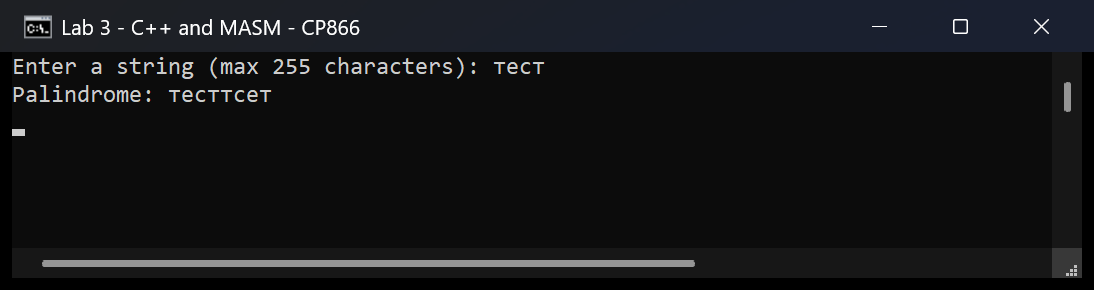
\includegraphics[width=\linewidth]{../tests/screenshots/11-russian.png}\\
\small Рисунок 1 --- Ввод и вывод русской строки в CP866
\end{center}

\section*{5 Код программы}
\noindent\textbf{Модуль C++ --- main.cpp}
\lstinputlisting[language=C++]{../code/main.cpp}

\newpage
\noindent\textbf{Модуль MASM --- palindrome.asm}
\lstinputlisting{../code/palindrome.asm}

\section*{6 Вывод}
Для вызова ассемблерной процедуры из C++ использованы три аргумента:
адрес исходной строки, адрес результата и длина. При \texttt{cdecl}
вызывающий код освобождает 12 байтов аргументов, поэтому в процедуре
достаточно \texttt{RET} без операнда. Регистры \texttt{ESI} и \texttt{EDI},
используемые цепочечными командами, восстанавливаются перед возвратом.
Сочетание \texttt{STD; LODSB; CLD; STOSB} позволяет читать строку
с конца и одновременно записывать её обратную копию вперёд.
\end{document}
